\documentclass{article}
\usepackage{graphicx}
\usepackage[margin=1.5cm]{geometry}
\usepackage{amsmath}

\begin{document}

\title{Wednesday Reading Assessment: Unit 1, Electric Fields}
\author{Prof. Jordan C. Hanson}

\maketitle

\section{Electric Fields}

\begin{enumerate}
\item Consider Fig. \ref{fig:ring} below.  A ring of charge with radius $R$ is situated in the xy-plane.  The charge is positive, and it is distributed evenly across the ring.  We write $dq = \lambda R d\theta$, to mean that there is $\lambda$ Coulombs per unit length.  If $d\theta$ were to extend to $2\pi$ (all the way around the circle), then the total charge is $Q = \lambda (2 \pi R)$.  (a) By symmetry, where should the electric field be zero?  (b) Where would the electric field be infinite?
\begin{figure}[ht]
\centering
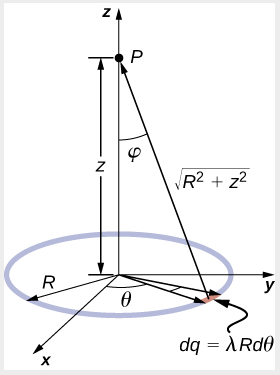
\includegraphics[width=0.22\textwidth]{ring.png}
\caption{\label{fig:ring} THings.}
\end{figure}
\item Consider again Fig. \ref{fig:ring}.  As $z \rightarrow \infty$, what happens to the field?
\begin{itemize}
\item A: The field-strength increases.
\item B: The field-strength remains constant.
\item C: The field-strength decreases.
\item D: The field-strength is exactly zero.
\end{itemize}
\item Suppose the actual function for the E-field $\vec{E}(z)$ is
\begin{equation}
\vec{E}(z) = \frac{1}{4\pi \epsilon_0} \frac{q z}{\left( z^2 + R^2 \right)^{3/2}} \hat{z}
\end{equation}
Evaluate the following limit:
\begin{equation}
\lim_{z \to \infty} \vec{E}(z) = \lim_{z \to \infty} \frac{1}{4\pi \epsilon_0} \frac{q z}{\left( z^2 + R^2 \right)^{3/2}} \hat{z}
\end{equation}
\textit{(Hint: it's not just zero.  Think about what the field should be if we observe it from far away).}
\end{enumerate}

\end{document}
